\documentclass[11pt,a4paper]{article}

\usepackage[margin=20mm,landscape]{geometry}
\usepackage{amsmath,amssymb,amsthm}
\usepackage{graphicx}
\usepackage{booktabs}
\usepackage{array}
\usepackage{xcolor}
\usepackage{microtype}
\usepackage[colorlinks=true,linkcolor=blue!55!black,urlcolor=blue!55!black]{hyperref}

\definecolor{ink}{HTML}{0B0B0B}
\definecolor{soft}{HTML}{52514E}
\definecolor{accent}{HTML}{2A78D6}
\definecolor{warn}{HTML}{D03B3B}

\newcommand{\T}{^{\mathsf{T}}}
\newcommand{\Lp}{L^{+}}
\newcommand{\note}[1]{{\color{soft}\small #1}}

% !TeX root = ../pipeline.tex
\newcommand{\gnb}{754}
\newcommand{\gne}{980}
\newcommand{\gnlines}{755}
\newcommand{\gntx}{225}
\newcommand{\gnwind}{157}
\newcommand{\gnwindgen}{425}
\newcommand{\gnPtdfEntries}{738,920}
\newcommand{\gnLpEntries}{568,516}
\newcommand{\grank}{750}
\newcommand{\gnullity}{4}
\newcommand{\growsum}{3.6e-10}
\newcommand{\gLone}{2.3e-10}
\newcommand{\gpsum}{1.6e-12}
\newcommand{\gpeffsum}{1.3e-12}
\newcommand{\gresid}{2.1e-09}
\newcommand{\gKdense}{0.27}
\newcommand{\gLdense}{0.46}
\newcommand{\gLpdense}{99.2}
\newcommand{\gnshift}{2}
\newcommand{\gshiftdeg}{17}
\newcommand{\gsnap}{2030-01-16 16:00:00}
\newcommand{\gworst}{1122-1742-1}
\newcommand{\gncong}{6}
\newcommand{\gncongtx}{0}
\newcommand{\gbmin}{-21638.3}
\newcommand{\gbmax}{1754386.0}
\newcommand{\gptdfmin}{-1.2093}
\newcommand{\gptdfmax}{1.0105}
\newcommand{\gwinb}{10}
\newcommand{\gwine}{6}
\newcommand{\gnnonwind}{597}
\newcommand{\gnwindentries}{153,860}
\newcommand{\gcommute}{0.0e+00}

% !TeX root = ../pipeline.tex
% full dump not generated; run build.py --full-dump


\title{\textbf{Shift Factors on the Irish Transmission Grid}\\[2mm]
\large The DC pipeline in full: $K$, $B$, $L$, $\Lp$, PTDF, sensitivity}
\author{Szymon Ablewicz \quad---\quad Team 6, Electrical Grid Hackathon 2026}
\date{Network: \texttt{WP2033\_all-island} \quad
      $\gnb$ buses, $\gne$ branches, $\gnwind$ wind nodes}

\begin{document}
\maketitle

\begin{abstract}
\noindent
Every matrix in this document is from the real all-island network:
$\gnb$ buses, $\gne$ branches ($\gnlines$ lines and $\gntx$ transformers),
$\gnwindgen$ wind farms at $\gnwind$ buses. Nothing here is a reduced example.

The pipeline computes, for every transmission branch $e$ and every wind node
$n$, how much the flow on $e$ changes per MW curtailed at $n$ --- the quantity
EirGrid calls a \emph{shift factor}. The result is a
$\gne \times \gnb$ matrix of $\gnPtdfEntries$ entries, exact to the DC model
rather than estimated.

\medskip\noindent
\textbf{On displaying the matrices.} $\Lp$ alone holds $\gnLpEntries$ entries
and is $\gLpdense\%$ dense. \TeX{} cannot typeset a $\gne$-column array --- it
exhausts its column registers long before it runs out of paper. So each matrix
appears twice: as a \emph{heatmap of the whole thing}, every entry present as
a pixel; and as a \emph{labelled numeric window} carrying real values at real
buses. Appendix~\ref{app:dump} holds the complete entry-by-entry dumps.
\end{abstract}

\vspace{2mm}
\begin{center}\small
\begin{tabular}{llll}
\toprule
\textbf{check} & \textbf{value} & \textbf{must be} & \textbf{meaning}\\
\midrule
flows vs.\ PyPSA \texttt{n.lpf()} & $\gresid$ MW & $\approx 0$ & an independent DC solver agrees\\
PTDF row sums & $\growsum$ & $0$ & 1\,MW at every bus at once moves nothing\\
$\|L\mathbf{1}\|_\infty$ & $\gLone$ & $0$ & the constant vector is in the nullspace\\
$\mathbf{1}\T p$ & $\gpsum$ & $0$ & injections balance\\
$\mathbf{1}\T p_{\text{eff}}$ & $\gpeffsum$ & $0$ & the phase-shift term preserves that\\
\bottomrule
\end{tabular}
\end{center}

\newpage
\section{The model: DC power flow}

The AC power-flow equations are nonlinear. The DC approximation linearises them
under three assumptions:
\begin{enumerate}\itemsep0pt
  \item every bus voltage magnitude is held at $1$ per unit;
  \item branch resistance is negligible beside reactance, $r \ll x$, so losses vanish;
  \item angle differences across branches are small, so $\sin(\theta_i-\theta_j)\approx\theta_i-\theta_j$.
\end{enumerate}

Active power flow on a branch then becomes exactly linear in the angle difference:
\begin{equation}
  f_e \;=\; \frac{\theta_{i(e)} - \theta_{j(e)}}{x_e}
       \;=\; b_e\,(\theta_{i} - \theta_{j}),
  \qquad b_e \equiv 1/x_e .
\end{equation}

\textbf{Why this matters.} Linearity is the whole reason a closed-form
sensitivity exists. In full AC one would perturb an injection and re-solve a
nonlinear system once per wind node --- which is what EirGrid's load-flow tool
does. In DC the derivative is exact, analytic, and available for every
branch--node pair at once from a single inversion.

\medskip
\textbf{What it is, in circuit terms.} Under DC the grid is an ordinary
resistive network and this is plain nodal analysis:

\begin{center}\small
\begin{tabular}{ll}
\toprule
circuit theory & DC power flow\\
\midrule
node voltage & bus voltage angle $\theta$\\
conductance $G = 1/R$ & susceptance $b = 1/x$\\
injected current source & net power injection $p$ (MW)\\
nodal conductance matrix $\mathbf{G}$ & $L = K B K\T$\\
$\mathbf{G}V = I$ (KCL at every node) & $L\theta = p$\\
Ohm's law on a branch & $f = B K\T \theta$\\
\bottomrule
\end{tabular}
\end{center}

\medskip
\textbf{What is given up.} No reactive power: real thermal limits are current
limits and current tracks $|S| = \sqrt{P^2+Q^2}$, while DC sees only $P$. And
no voltage-stability representation at all --- several real EirGrid constraint
groups exist for exactly that reason and are outside anything computed here.

\newpage
\section{Stage 1 --- build \texorpdfstring{$K$, $B$, $\varphi$, $L$}{K, B, phi, L}}

\subsection*{$K$, the bus--branch incidence matrix \quad $\gnb \times \gne$}

Column $e$ has exactly two non-zeros: $+1$ in the row of the branch's
\texttt{bus0}, $-1$ in the row of its \texttt{bus1}.
\[
  K_{ie} =
  \begin{cases}
    +1 & i = \text{bus0}(e)\\
    -1 & i = \text{bus1}(e)\\
    0  & \text{otherwise.}
  \end{cases}
\]
This is topology only --- which buses connect to which --- and carries no
electrical information. It is $\gKdense\%$ dense.

\textbf{The orientation is arbitrary.} Which end is called \texttt{bus0} was
decided by row order in the data file. Harmless through Stage 3; Stage 4 exists
to clean it up.

\begin{center}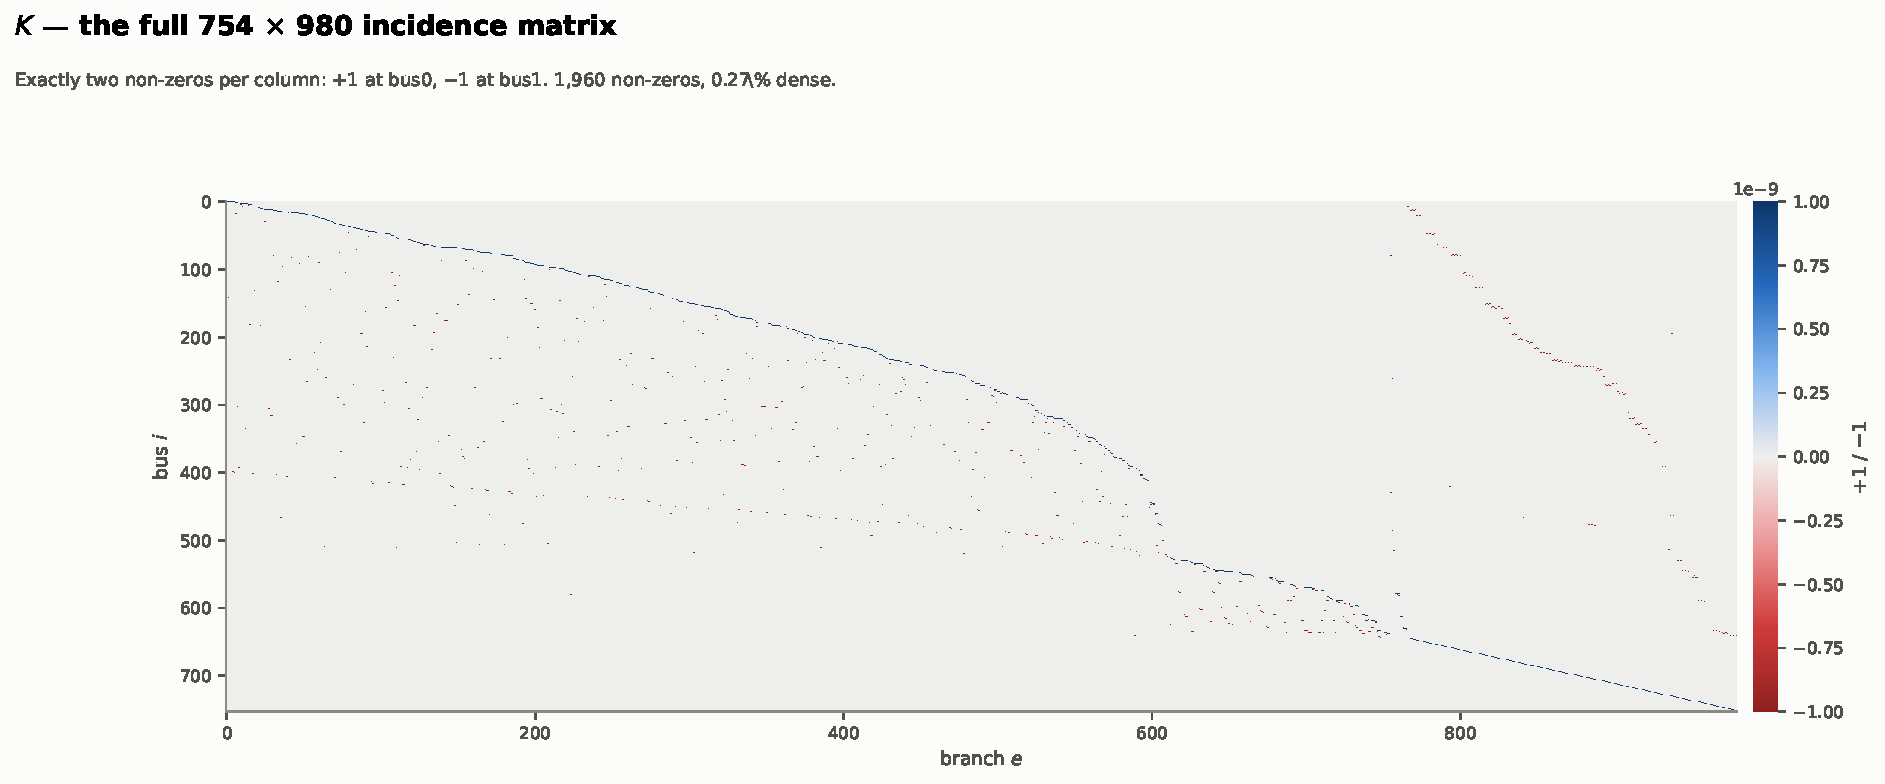
\includegraphics[width=\linewidth]{figures/m_K}\end{center}

\newpage
\subsection*{$K$ --- real entries}

$\gwinb$ buses against the $\gwine$ congested branches. Every column shows the
same $+1/-1$ pair.
\begin{center}% !TeX root = ../pipeline.tex
\setlength{\tabcolsep}{3pt}\renewcommand{\arraystretch}{1.05}
\begin{tabular}{l|rrrrrr}
{\tiny bus / branch} & {\tiny 1122-1742-1} & {\tiny 1122-11260-1} & {\tiny 2781-4951-1} & {\tiny 3082-3122-1} & {\tiny 3581-89516-1} & {\tiny 3691-4041-1}\\ \hline
{\tiny ARKLOW} & $1$ & $1$ & $0$ & $0$ & $0$ & $0$\\
{\tiny CARRICKMINES} & $-1$ & $0$ & $0$ & $0$ & $0$ & $0$\\
{\tiny GALWAY} & $0$ & $0$ & $1$ & $0$ & $0$ & $0$\\
{\tiny INCHICORE} & $0$ & $0$ & $0$ & $1$ & $0$ & $0$\\
{\tiny IRISHTOWN} & $0$ & $0$ & $0$ & $-1$ & $0$ & $0$\\
{\tiny LETTERKENNY} & $0$ & $0$ & $0$ & $0$ & $1$ & $0$\\
{\tiny LAGHTANVACK} & $0$ & $0$ & $0$ & $0$ & $0$ & $1$\\
{\tiny MOY} & $0$ & $0$ & $0$ & $0$ & $0$ & $-1$\\
{\tiny SALTHILL} & $0$ & $0$ & $-1$ & $0$ & $0$ & $0$\\
{\tiny GLENART} & $0$ & $-1$ & $0$ & $0$ & $0$ & $0$
\end{tabular}
\end{center}

\subsection*{$B$, the susceptance matrix \quad $\gne \times \gne$ diagonal}

\[ B = \operatorname{diag}(b_1,\dots,b_{\gne}), \qquad b_e = 1/x_e \]
in MW per radian, ranging from $\gbmin$ to $\gbmax$ across the network. For the
congested branches:
\[ B_{\text{cong}} = % !TeX root = ../pipeline.tex
\operatorname{diag}\big(2192.0,\; 58823.5,\; 37092.0,\; 21285.7,\; 1307.2,\; 1109.9\big)
 \]

\note{PyPSA stores per-unit reactance on a 1\,MVA base, so $1/x_{\text{pu}}$ is
already in MW/rad --- verified directly: for line \texttt{1021-2121-1},
$x = 7.634011\,\Omega$ at $110$\,kV gives
$x_{\text{pu}}\cdot v_{\text{nom}}^2 / x = 1.000$\,MVA exactly.}

\subsection*{$\varphi$, the phase shifts \quad $\gne$ vector, radians}

Zero for every line and every ordinary transformer. Non-zero for exactly
$\gnshift$ phase-shifting transformers, the larger at $\gshiftdeg^\circ$. A
shifter imposes an angle of its own, so its flow is
$f_e = b_e(\theta_i - \theta_j - \varphi_e)$. It does not enter until Stage 4.

\newpage
\subsection*{$L = K B K\T$, the weighted Laplacian \quad $\gnb \times \gnb$}

\[
  L_{ij} =
  \begin{cases}
    \sum_{e \ni i} b_e & i = j\\
    -\,b_e & i \neq j,\ \text{branch } e \text{ joins } i,j\\
    0 & \text{otherwise}
  \end{cases}
\]

This is the DC bus admittance matrix. Applying it to the angle vector gives
\begin{equation}
  L\theta = p,
\end{equation}
which is \textbf{Kirchhoff's Current Law written at every bus at once}: net
power injected at a bus equals the power flowing out along its branches.

$L$ is $\gLdense\%$ dense --- it inherits the grid's own sparsity, because
$L_{ij}\neq 0$ only for buses that are physically connected.

\begin{center}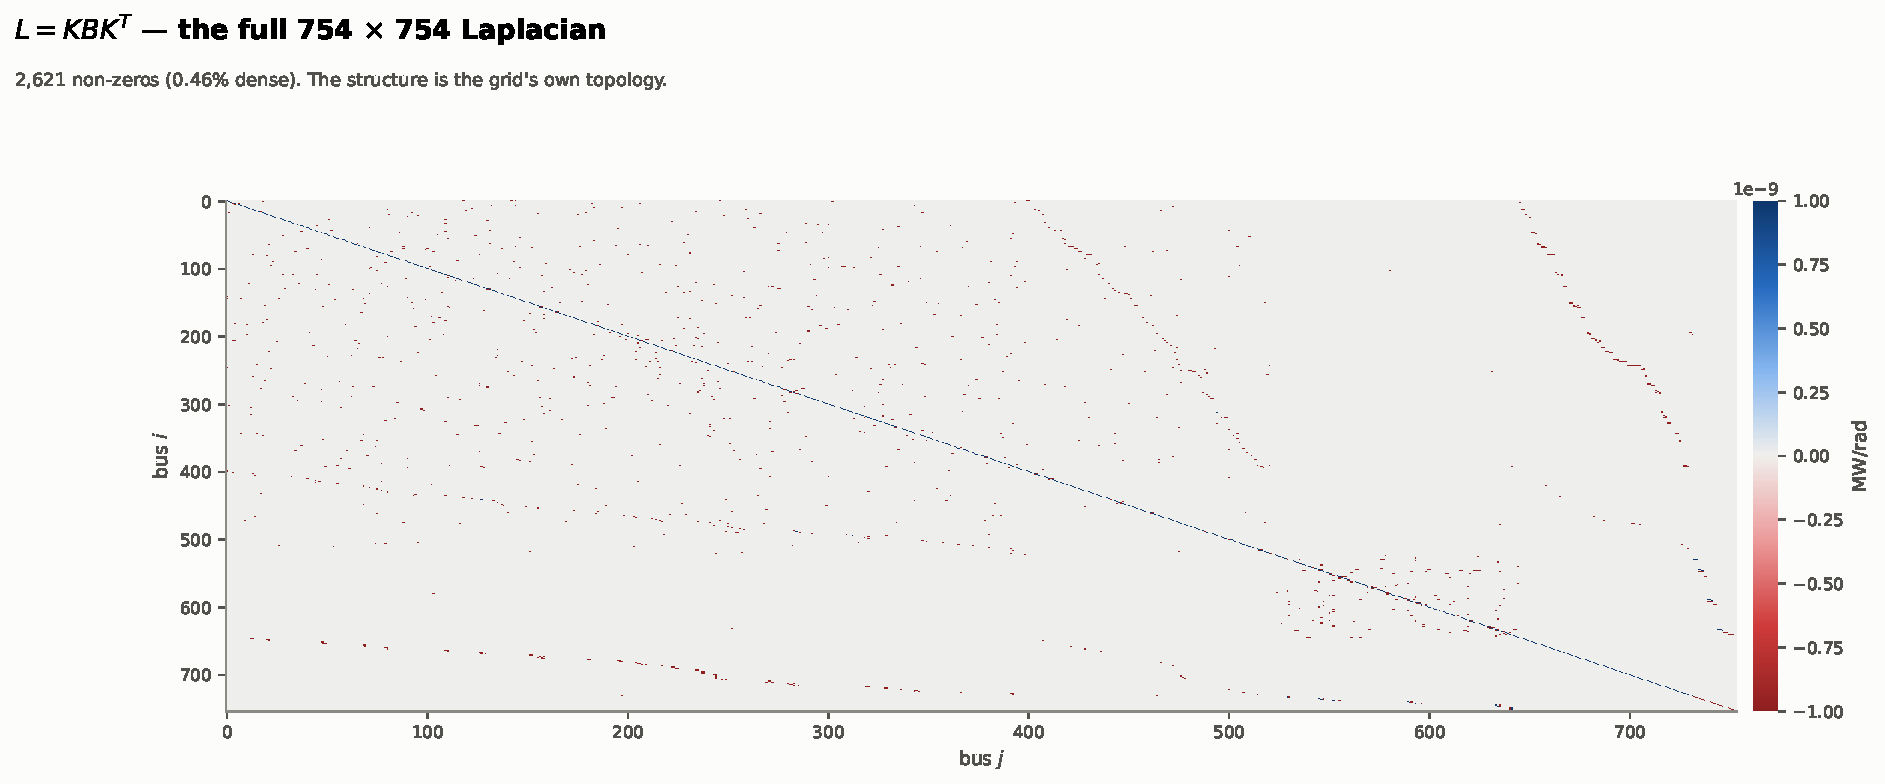
\includegraphics[width=\linewidth]{figures/m_L}\end{center}

\newpage
\subsection*{$L$ --- real entries \quad ($\times 10^{3}$ MW/rad)}

\begin{center}% !TeX root = ../pipeline.tex
\setlength{\tabcolsep}{3pt}\renewcommand{\arraystretch}{1.05}
\begin{tabular}{l|rrrrrrrrrr}
{\tiny } & {\tiny ARKLOW} & {\tiny CARRICKMINES} & {\tiny GALWAY} & {\tiny INCHICORE} & {\tiny IRISHTOWN} & {\tiny LETTERKENNY} & {\tiny LAGHTANVACK} & {\tiny MOY} & {\tiny SALTHILL} & {\tiny GLENART}\\ \hline
{\tiny ARKLOW} & $67.93$ & $-2.19$ & $0$ & $0$ & $0$ & $0$ & $0$ & $0$ & $0$ & $-58.82$\\
{\tiny CARRICKMINES} & $-2.19$ & $1093.29$ & $0$ & $0$ & $-21.59$ & $0$ & $0$ & $0$ & $0$ & $0$\\
{\tiny GALWAY} & $0$ & $0$ & $47.98$ & $0$ & $0$ & $0$ & $0$ & $0$ & $-37.09$ & $0$\\
{\tiny INCHICORE} & $0$ & $0$ & $0$ & $1035.67$ & $-21.29$ & $0$ & $0$ & $0$ & $0$ & $0$\\
{\tiny IRISHTOWN} & $0$ & $-21.59$ & $0$ & $-21.29$ & $209.55$ & $0$ & $0$ & $0$ & $0$ & $0$\\
{\tiny LETTERKENNY} & $0$ & $0$ & $0$ & $0$ & $0$ & $1019.00$ & $0$ & $0$ & $0$ & $0$\\
{\tiny LAGHTANVACK} & $0$ & $0$ & $0$ & $0$ & $0$ & $0$ & $42.78$ & $-1.11$ & $0$ & $0$\\
{\tiny MOY} & $0$ & $0$ & $0$ & $0$ & $0$ & $0$ & $-1.11$ & $2011.92$ & $0$ & $0$\\
{\tiny SALTHILL} & $0$ & $0$ & $-37.09$ & $0$ & $0$ & $0$ & $0$ & $0$ & $40.10$ & $0$\\
{\tiny GLENART} & $-58.82$ & $0$ & $0$ & $0$ & $0$ & $0$ & $0$ & $0$ & $0$ & $105.34$
\end{tabular}
\end{center}

\note{Diagonal entries sum over \emph{all} branches at that bus, including ones
leaving this window --- so a diagonal here can exceed the off-diagonals shown.
That is the one thing a window cannot show, and is why the heatmap above
accompanies it.}

\subsection*{Scale invariance}

\textbf{Claim.} PTDF is unchanged if every susceptance is multiplied by a
constant $c$.

\textbf{Proof.} Let $B \to cB$. Then $L \to cL$, and $\Lp \to \Lp/c$ by the
Moore--Penrose property of scalar multiples, so
\[
  \text{PTDF} = (cB)K\T\!\left(\tfrac{1}{c}\Lp\right) = B K\T \Lp . \qquad\blacksquare
\]

So the PTDF needs no MVA base. \textbf{This does not extend to Stage 4}: there
$p_{\text{eff}} = p + KB\varphi$ \emph{adds} a $B$-weighted term to a vector in
MW, so once $\varphi \neq 0$, $B$ must be in genuine MW/radian.

\newpage
\section{Stage 2 --- the Moore--Penrose pseudoinverse}

\subsection*{Why $L$ cannot be inverted}

Every column of $K$ has one $+1$ and one $-1$, so
\begin{equation}
  K\T\mathbf{1} = \mathbf{0}
  \quad\Longrightarrow\quad
  L\mathbf{1} = K B (K\T \mathbf{1}) = \mathbf{0}.
\end{equation}
The all-ones vector is in the nullspace: adding the same angle to every bus
changes no flow. Measured, $\|L\mathbf{1}\|_\infty = \gLone$.

Here $\operatorname{rank}(L) = \grank$ of $\gnb$, so the nullity is $\gnullity$ ---
one dimension per connected component. The extra three are the AC-isolated far
terminals of the DC links (Moyle's Scotland end, \texttt{GB\_EWIC},
\texttt{GB\_GREENLINK}); a DC link is a controllable injection, not a branch,
so it never enters $K$.

\subsection*{What Moore--Penrose gives}

$\Lp$ is the unique matrix satisfying Penrose's four conditions. What matters
here is that it inverts $L$ on the orthogonal complement of the nullspace and
returns the \textbf{minimum-norm} solution --- so $\theta = \Lp p$ satisfies
$\mathbf{1}\T\theta = 0$.

\textbf{This is not a workaround for the singularity; it is a choice of
reference, made explicit.} The textbook alternative deletes a slack row and
column, which writes an arbitrary choice into every number that follows.

\subsection*{Why it amounts to uniform distributed slack}

Inject 1\,MW at bus $n$ and withdraw it evenly everywhere:
$p = e_n - \tfrac{1}{N}\mathbf{1}$. Since $\Lp\mathbf{1} = \mathbf{0}$,
\begin{equation}
  \Lp p = \Lp e_n - \tfrac{1}{N}\Lp\mathbf{1} = \Lp e_n .
\end{equation}
So reading column $n$ of $\Lp$ \emph{is} injecting at $n$ against a uniform
distributed slack. \qed{}

\newpage
\subsection*{$\Lp$ --- the whole thing, and why it is expensive}

\begin{center}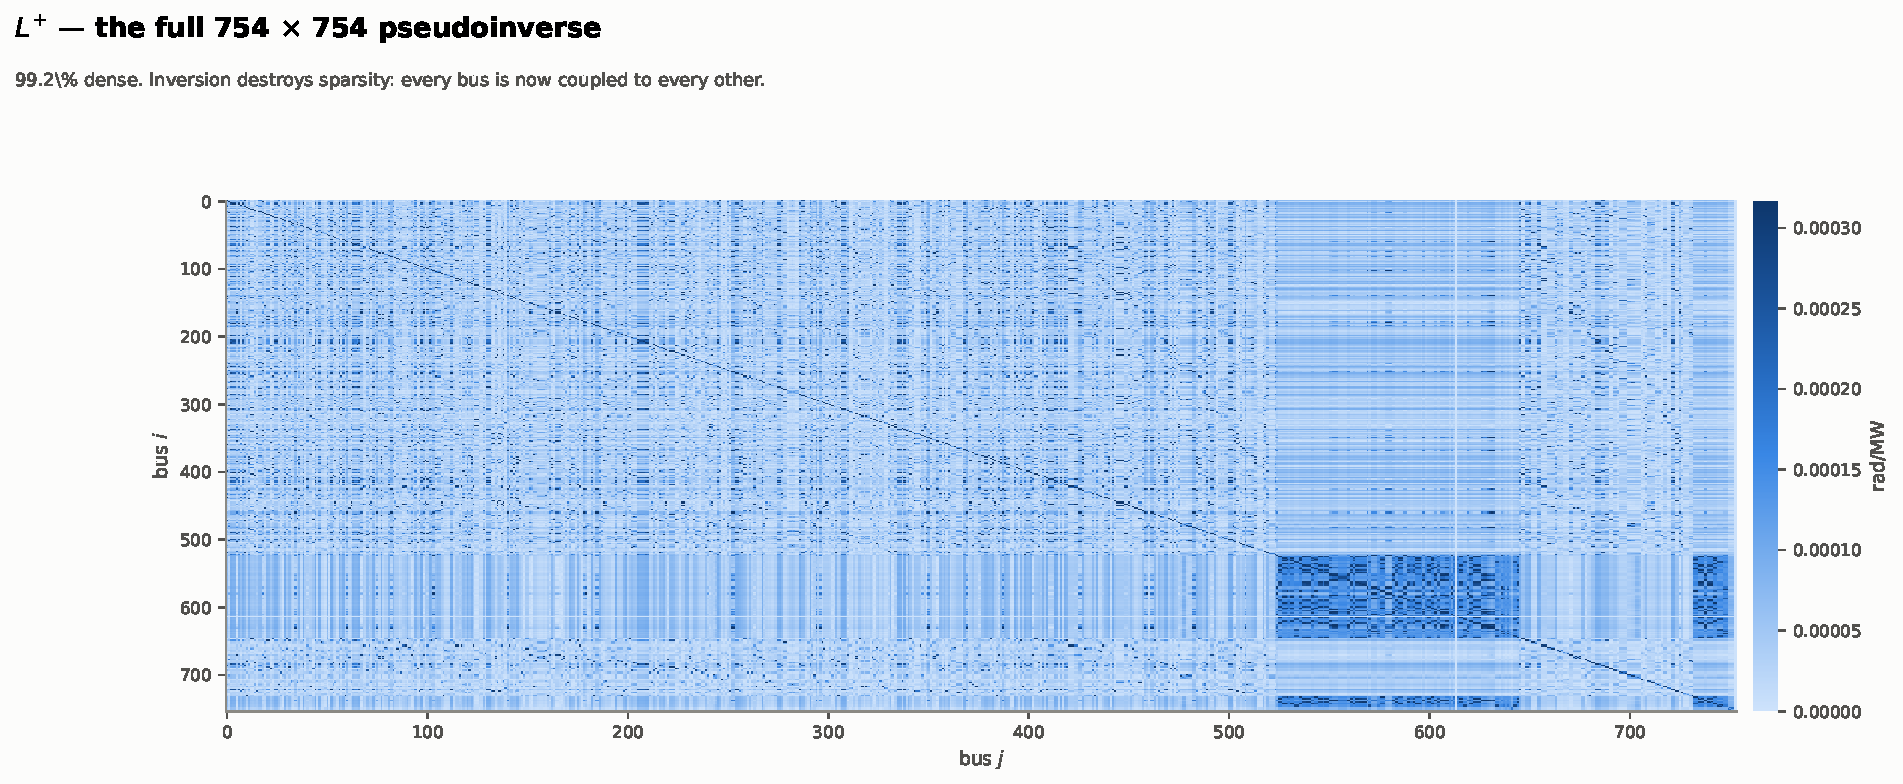
\includegraphics[width=\linewidth]{figures/m_Lp}\end{center}

\medskip
$L$ is $\gLdense\%$ dense. $\Lp$ is $\gLpdense\%$ dense.
\textbf{Inversion destroys sparsity} --- every bus becomes coupled to every
other --- which is why this single SVD is the only expensive step in the
pipeline. It is done once and reused for every branch, every wind node and
every snapshot.

\subsection*{$\Lp$ --- real entries \quad ($\times 10^{-4}$ rad/MW)}

\begin{center}% !TeX root = ../pipeline.tex
\setlength{\tabcolsep}{3pt}\renewcommand{\arraystretch}{1.05}
\begin{tabular}{l|rrrrrrrrrr}
{\tiny } & {\tiny ARKLOW} & {\tiny CARRICKMINES} & {\tiny GALWAY} & {\tiny INCHICORE} & {\tiny IRISHTOWN} & {\tiny LETTERKENNY} & {\tiny LAGHTANVACK} & {\tiny MOY} & {\tiny SALTHILL} & {\tiny GLENART}\\ \hline
{\tiny ARKLOW} & $3.386$ & $0.896$ & $-0.301$ & $0.568$ & $0.732$ & $-0.745$ & $-0.590$ & $-0.594$ & $-0.303$ & $3.385$\\
{\tiny CARRICKMINES} & $0.896$ & $1.372$ & $-0.232$ & $0.930$ & $1.152$ & $-0.585$ & $-0.482$ & $-0.474$ & $-0.234$ & $0.895$\\
{\tiny GALWAY} & $-0.301$ & $-0.232$ & $4.364$ & $-0.220$ & $-0.227$ & $-0.265$ & $1.341$ & $0.893$ & $4.321$ & $-0.302$\\
{\tiny INCHICORE} & $0.568$ & $0.930$ & $-0.220$ & $1.109$ & $1.018$ & $-0.552$ & $-0.459$ & $-0.448$ & $-0.221$ & $0.568$\\
{\tiny IRISHTOWN} & $0.732$ & $1.152$ & $-0.227$ & $1.018$ & $1.318$ & $-0.569$ & $-0.471$ & $-0.462$ & $-0.229$ & $0.732$\\
{\tiny LETTERKENNY} & $-0.745$ & $-0.585$ & $-0.265$ & $-0.552$ & $-0.569$ & $8.884$ & $0.574$ & $0.937$ & $-0.267$ & $-0.745$\\
{\tiny LAGHTANVACK} & $-0.590$ & $-0.482$ & $1.341$ & $-0.459$ & $-0.471$ & $0.574$ & $12.671$ & $7.643$ & $1.339$ & $-0.591$\\
{\tiny MOY} & $-0.594$ & $-0.474$ & $0.893$ & $-0.448$ & $-0.462$ & $0.937$ & $7.643$ & $10.029$ & $0.891$ & $-0.595$\\
{\tiny SALTHILL} & $-0.303$ & $-0.234$ & $4.321$ & $-0.221$ & $-0.229$ & $-0.267$ & $1.339$ & $0.891$ & $4.540$ & $-0.303$\\
{\tiny GLENART} & $3.385$ & $0.895$ & $-0.302$ & $0.568$ & $0.732$ & $-0.745$ & $-0.591$ & $-0.595$ & $-0.303$ & $3.555$
\end{tabular}
\end{center}

\newpage
\section{Stage 3 --- the PTDF}

\begin{equation}
  \boxed{\;\text{PTDF} \;=\; B K\T \Lp\;}
  \qquad
  \underbrace{(\gne \times \gne)}_{B}
  \underbrace{(\gne \times \gnb)}_{K\T}
  \underbrace{(\gnb \times \gnb)}_{\Lp}
  \;\longrightarrow\; \gne \times \gnb
\end{equation}

Read as two composed steps:
\[
  \text{PTDF} \;=\; \underbrace{B K\T}_{\text{angles}\,\to\,\text{flows}}
                \cdot \underbrace{\Lp}_{\text{injections}\,\to\,\text{angles}}
\]
$\Lp$ solves the network; $B K\T$ reads flows off the angles, since $K\T\theta$
is the angle difference across each branch and multiplying by $1/x$ is Ohm's
law. Pre-multiplying them means the network is never solved again.

\subsection*{What one entry means}
\[
  \text{PTDF}_{en} \;=\;
  \frac{\partial f_e}{\partial p_n}
  \;=\;
  \begin{minipage}{0.5\linewidth}
  change in flow on branch $e$, in MW, per MW injected at bus $n$, with the
  balancing withdrawal spread uniformly.
  \end{minipage}
\]
Dimensionless --- MW per MW\@. Here it spans $[\gptdfmin, \gptdfmax]$.
\textbf{It is the exact analytic derivative of the model, not a
finite-difference estimate}; every one of the $\gnPtdfEntries$ entries falls out
of the single inversion in Stage 2.

\subsection*{The check that costs nothing}
\begin{equation}
  \sum_{n} \text{PTDF}_{en} = 0 \quad \text{for every } e,
\end{equation}
because injecting 1\,MW at every bus simultaneously moves no power.
Measured: $\growsum$.

\newpage
\begin{center}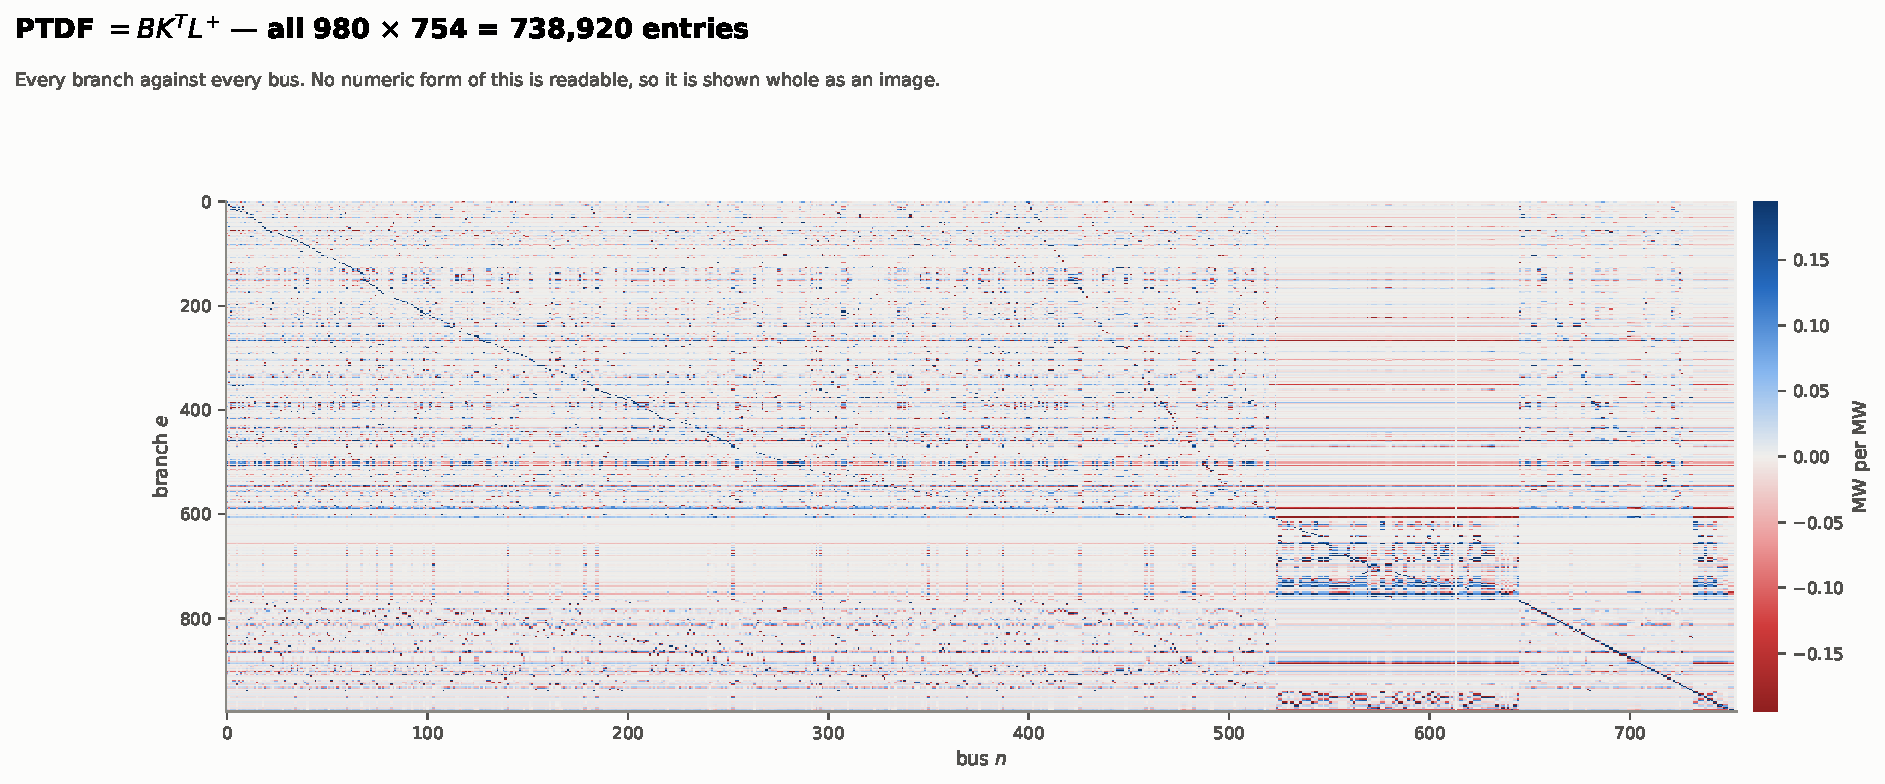
\includegraphics[width=\linewidth]{figures/m_PTDF}\end{center}

\subsection*{PTDF --- real entries}

The $\gwine$ congested branches against ten buses. A star marks a bus with wind
on it; the rest are load, conventional generation, or bare junctions.
\begin{center}% !TeX root = ../pipeline.tex
\setlength{\tabcolsep}{3pt}\renewcommand{\arraystretch}{1.05}
\begin{tabular}{l|rrrrrrrrrr}
{\tiny branch / bus} & {\tiny ARDNACRUSHA*} & {\tiny BALRUNTAGH} & {\tiny ARIGNA*} & {\tiny AGHADA} & {\tiny ARKLOW*} & {\tiny AGHADA} & {\tiny ATHEA*} & {\tiny AGHADA\_B} & {\tiny ATHLONE*} & {\tiny AGH\_AT14}\\ \hline
{\tiny 1122-1742-1} & $0.0187$ & $-0.0406$ & $-0.0295$ & $0.0707$ & $0.4516$ & $0.0706$ & $0.0004$ & $0.0706$ & $-0.0109$ & $0.0706$\\
{\tiny 1122-11260-1} & $0.0027$ & $0.0027$ & $0.0027$ & $0.0027$ & $0.0027$ & $0.0027$ & $0.0027$ & $0.0027$ & $0.0027$ & $0.0027$\\
{\tiny 2781-4951-1} & $0.0059$ & $0.0059$ & $0.0059$ & $0.0059$ & $0.0059$ & $0.0059$ & $0.0059$ & $0.0059$ & $0.0059$ & $0.0059$\\
{\tiny 3082-3122-1} & $-0.0128$ & $0.0494$ & $0.0335$ & $-0.0519$ & $-0.3496$ & $-0.0518$ & $-0.0050$ & $-0.0518$ & $0.0186$ & $-0.0518$\\
{\tiny 3581-89516-1} & $-0.0024$ & $0.0146$ & $0.0919$ & $-0.0054$ & $-0.0097$ & $-0.0055$ & $-0.0056$ & $-0.0055$ & $0.0135$ & $-0.0055$\\
{\tiny 3691-4041-1} & $0.0114$ & $-0.0231$ & $-0.0694$ & $0.0061$ & $0.0005$ & $0.0060$ & $0.0064$ & $0.0060$ & $0.0035$ & $0.0060$
\end{tabular}
\end{center}

\note{Both signs occur and both are meaningful. A negative entry means
injection at $n$ pushes flow in the \texttt{bus1}$\to$\texttt{bus0} direction
--- it does \emph{not} yet mean ``makes congestion worse''. That reading needs
Stage 4.}

\newpage
\section{Selecting the wind nodes}

PTDF has a column for every one of the $\gnb$ buses. Only $\gnwind$ of them
carry wind, and only wind can be curtailed --- so the $\gnnonwind$ remaining
columns are not part of any curtailment decision.

\textbf{This is a column selection and nothing more.} Write $S$ for the
$\gnb \times \gnwind$ matrix with a single $1$ in each column, at the row of
that wind bus:
\begin{equation}
  \text{PTDF}_{\text{wind}} \;=\; \text{PTDF} \cdot S,
  \qquad
  S \in \{0,1\}^{\gnb \times \gnwind},
  \qquad
  \gne \times \gnb \;\longrightarrow\; \gne \times \gnwind .
\end{equation}
No arithmetic happens. Nothing is recomputed. In code it is
\texttt{ptdf[:, wind\_buses]}.

\subsection*{Why the other \texorpdfstring{$\gnnonwind$}{597} buses cannot be dropped earlier}

They are not padding --- they are the network the power flows \emph{through}.
Column $n$ of PTDF is $B K\T (\Lp e_n)$, and $\Lp e_n$ is the whole network's
response to an injection at $n$. That response depends on every bus and every
branch. \textbf{There is no $\gnwind \times \gnwind$ Laplacian to build}:
delete the Dublin load buses and the Donegal wind columns change.

\medskip
So the selection has to come \emph{after} Stages 1--3, never before. One could
compute only the $\gnwind$ needed columns of $\Lp$ --- that is $\gnwind$
least-squares solves rather than a full pseudoinverse --- but on a
$\gnb \times \gnb$ matrix the full \texttt{pinv} takes under a second, and
computing all of it buys the row-sum check across every bus for free.

\note{Kron reduction onto the wind buses would also be wrong here. It preserves
behaviour at the retained buses but discards flows on the eliminated branches
--- and every branch is monitored, including the $\gncongtx$ congested
transformers.}

\subsection*{Selection and the sign correction commute}

The sign correction of Stage 4 scales each \emph{row}; the selection keeps
certain \emph{columns}. Row scaling and column selection act on different
indices, so
\begin{equation}
  \big(\operatorname{diag}(\sigma)\,\text{PTDF}\big) S
  \;=\;
  \operatorname{diag}(\sigma)\,\big(\text{PTDF}\,S\big),
  \qquad \sigma_e = \operatorname{sign}(f_e).
\end{equation}
Verified numerically: the two orderings differ by $\gcommute$. The code slices
first and signs second; this document signs first and slices second. Same
matrix either way.

\begin{center}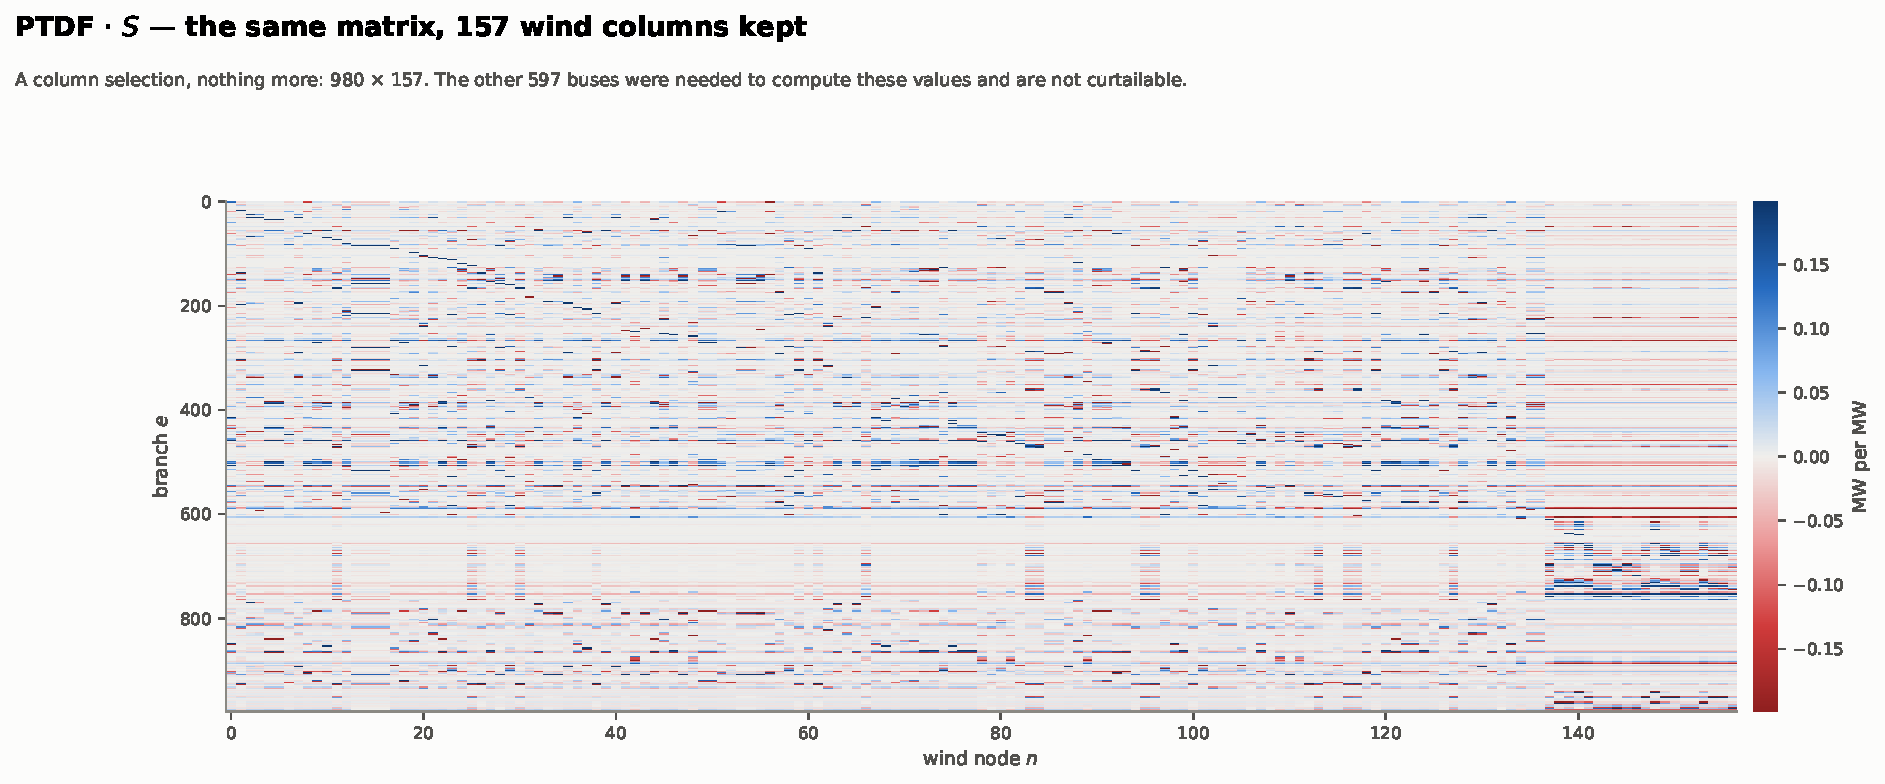
\includegraphics[width=\linewidth]{figures/m_PTDFwind}\end{center}

\subsection*{$\text{PTDF}\cdot S$ --- real entries}

The same $\gwine$ congested branches, now against wind nodes only:
\begin{center}\input{generated/w_PTDF}\end{center}

\newpage
\section{Stage 4 --- correct the sign direction}

\subsection*{The problem}

Two quantities sit on the \emph{same arbitrary axis} set by the \texttt{bus0}/
\texttt{bus1} labelling: the base flow $f_e$, and the row $\text{PTDF}_{e,:}$.
That axis came from data-file row order.

Congestion, however, is about \emph{magnitude} --- $|f|$ against the rating:

\begin{center}\small
\begin{tabular}{lll}
\toprule
base flow on $e$ & overload means & relief requires\\
\midrule
positive (bus0$\to$bus1) & $f$ too large positive & $\text{PTDF}_{en} > 0$\\
negative (bus1$\to$bus0) & $f$ too large negative & $\text{PTDF}_{en} < 0$\\
\bottomrule
\end{tabular}
\end{center}

\textbf{So the sign meaning ``relieves congestion'' flips with an arbitrary
labelling choice.} Roughly half of all branches are affected, and a
sign-flipped ranking looks entirely plausible on inspection.

\subsection*{Getting $f$ right: the phase-shift term}

A phase shifter imposes its own angle, so $f = B(K\T\theta - \varphi)$. KCL
still gives $Kf = p$, so
\begin{align}
  K B (K\T\theta - \varphi) &= p\\
  L\theta &= p + KB\varphi .
\end{align}
The shifter appears exactly where an injection would --- \textbf{it behaves as
a pair of equal and opposite injections at its two ends.} Define
$p_{\text{eff}} = p + KB\varphi$; then

\begin{equation}
  \boxed{\;\theta = \Lp p_{\text{eff}}, \qquad
  f = B K\T\theta - B\varphi = \text{PTDF}\cdot p_{\text{eff}} - B\varphi\;}
\end{equation}

Same $\Lp$, same PTDF, one modified input vector and one constant subtraction.

\textbf{Three properties.}
\emph{(i)} $\mathbf{1}\T p_{\text{eff}} = \mathbf{1}\T p + (K\T\mathbf{1})\T
B\varphi = 0$, so balance survives --- measured $\gpeffsum$.
\emph{(ii)} Expanding, $f = \text{PTDF}\cdot p + c$ with
$c = (BK\T\Lp K - I)B\varphi$ independent of $p$: a constant offset, not a
different model.
\emph{(iii)} At $\varphi = 0$ it reduces term by term to $f = \text{PTDF}\cdot p$.

\medskip
\textbf{PTDF is untouched by any of this:}
$\partial f/\partial p = \text{PTDF}\cdot \partial p_{\text{eff}}/\partial p =
\text{PTDF}$, because $\varphi$ is a fixed device setting, not a function of
injection.

\newpage
\subsection*{Why the term is not optional}

This network has $\gnshift$ phase shifters, one at $\gshiftdeg^\circ$. Dropping
$B\varphi$ leaves the most heavily loaded circuit in the network,
\texttt{3581-89516-1}, reading $44.2$\,MW against a $123$\,MVA rating --- $36\%$
loaded --- when it is in fact at $123.0$\,MW, \textbf{exactly at its limit}.
It stops looking congested at all. Across the network, $272$ of $\gne$ branches
come out wrong by more than 1\,MW, worst case $78.8$\,MW.

\subsection*{The fix}

\begin{equation}
  \boxed{\;\text{sensitivity}_{e,:} \;=\; \text{PTDF}_{e,:}\cdot
  \operatorname{sign}(f_e)\;}
\end{equation}

\begin{center}\small
\begin{tabular}{ll}
\toprule
$\operatorname{sign}(f_e) = +1$ & axis already runs along the real flow; row unchanged\\
$\operatorname{sign}(f_e) = -1$ & axis runs backwards; row flipped\\
\bottomrule
\end{tabular}
\end{center}

\textbf{Verification against EirGrid's convention.} Let
$S = \text{PTDF}_{en}\operatorname{sign}(f_e)$. Reducing generation by $r>0$ at
$n$ is an injection change of $-r$, so the flow-aligned quantity changes by
$-Sr$:
\begin{itemize}\itemsep0pt
  \item $S>0$: change is negative, flow shrinks along its own direction,
        magnitude falls --- \textbf{congestion relieved}. \checkmark{}
  \item $S<0$: flow grows along its own direction, magnitude rises ---
        \textbf{congestion worsened}. \checkmark{}
\end{itemize}

\subsection*{Flows and signs --- real values at \texttt{\gsnap}}

\begin{center}% !TeX root = ../pipeline.tex
\setlength{\tabcolsep}{3pt}\renewcommand{\arraystretch}{1.05}
\begin{tabular}{l|rrr}
{\tiny branch} & {\tiny f (MW)} & {\tiny sign} & {\tiny peak load \%} \tabularnewline \hline
{\tiny 1122-1742-1} & $281.79$ & $1.00$ & $100.00$\\
{\tiny 1122-11260-1} & $-228.78$ & $-1.00$ & $100.00$\\
{\tiny 2781-4951-1} & $-64.15$ & $-1.00$ & $100.00$\\
{\tiny 3082-3122-1} & $-378.14$ & $-1.00$ & $100.00$\\
{\tiny 3581-89516-1} & $123.00$ & $1.00$ & $100.00$\\
{\tiny 3691-4041-1} & $81.00$ & $1.00$ & $100.00$
\end{tabular}
\end{center}

\note{This is the only snapshot-dependent step. Stages 1--3 depend on topology
and reactance alone and hold for every hour of the year. Measured across all
168 snapshots, a branch's sign agrees with its own peak-hour sign $98.6\%$ of
the time when it is above $50\%$ loaded ($87.4\%$ at worst).}

\newpage
\section{The result}

\begin{center}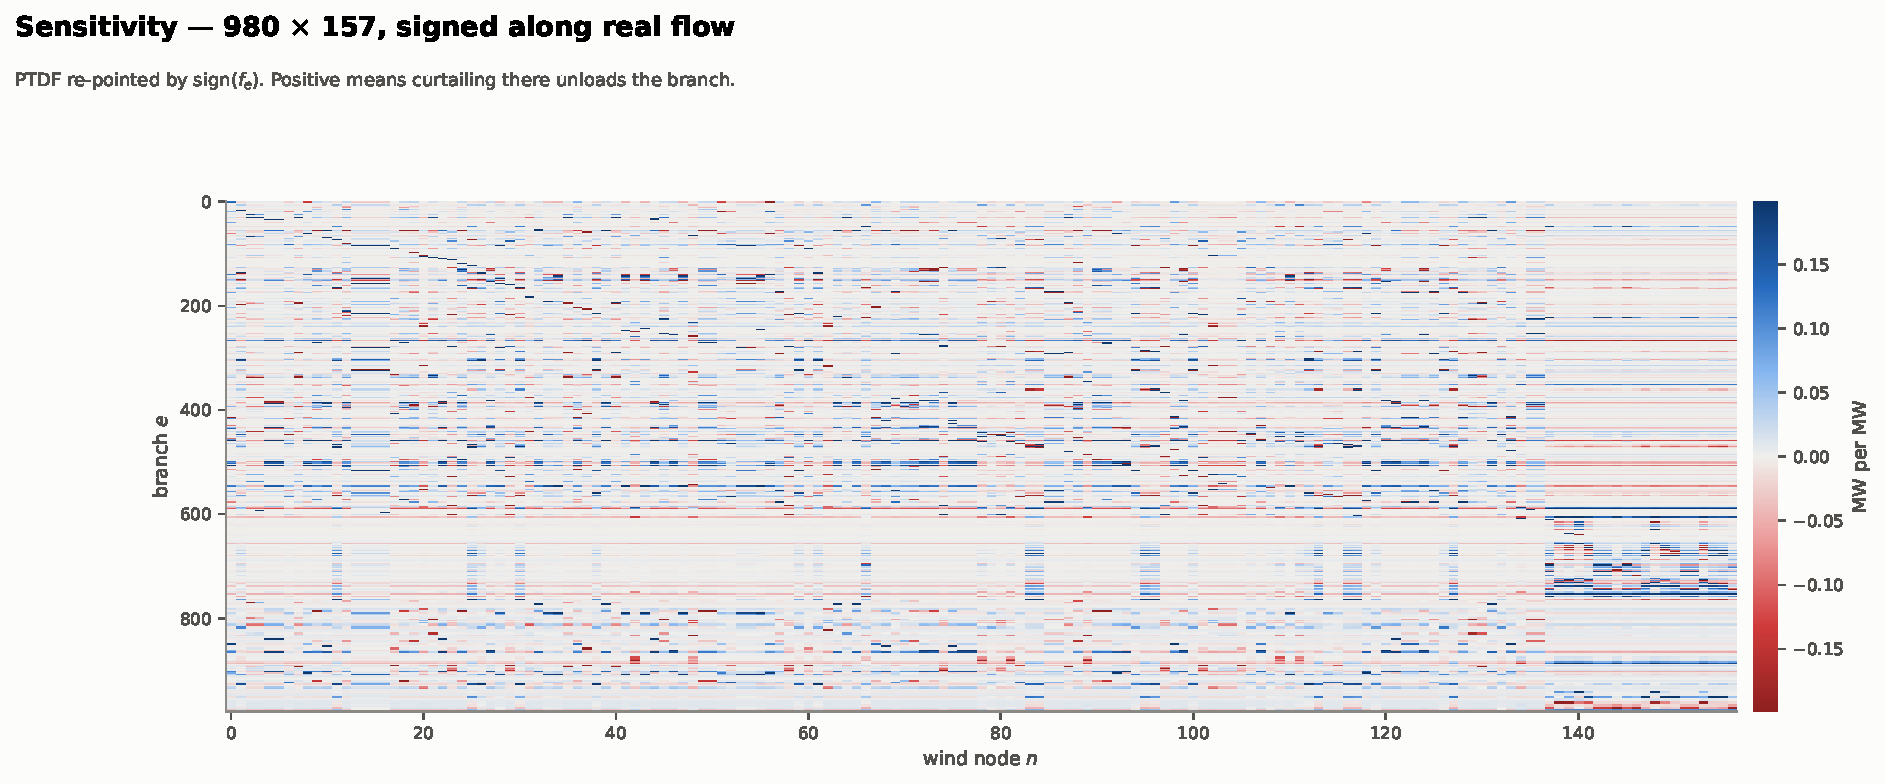
\includegraphics[width=\linewidth]{figures/m_sens}\end{center}

\subsection*{Sensitivity --- real entries}

\begin{center}% !TeX root = ../pipeline.tex
\setlength{\tabcolsep}{3pt}\renewcommand{\arraystretch}{1.05}
\begin{tabular}{l|rrrrrrrrrr}
{\tiny branch / wind bus} & {\tiny ARDNACRUSHA} & {\tiny ARIGNA} & {\tiny ARKLOW} & {\tiny W\_ARKLOW\_OFF} & {\tiny ATHEA} & {\tiny TOBERTOREEN} & {\tiny ATHLONE} & {\tiny BALLYWATER} & {\tiny BOOLTIAGH} & {\tiny BALLYLICKEY}\\ \hline
{\tiny 1122-1742-1} & $0.0187$ & $-0.0295$ & $0.4516$ & $0.5458$ & $0.0004$ & $0.0004$ & $-0.0109$ & $0.3563$ & $0.0026$ & $0.0559$\\
{\tiny 1122-11260-1} & $-0.0027$ & $-0.0027$ & $-0.0027$ & $0.9973$ & $-0.0027$ & $-0.0027$ & $-0.0027$ & $-0.0027$ & $-0.0027$ & $-0.0027$\\
{\tiny 2781-4951-1} & $-0.0059$ & $-0.0059$ & $-0.0059$ & $-0.0059$ & $-0.0059$ & $-0.0059$ & $-0.0059$ & $-0.0059$ & $-0.0059$ & $-0.0059$\\
{\tiny 3082-3122-1} & $0.0128$ & $-0.0335$ & $0.3496$ & $0.3495$ & $0.0050$ & $0.0050$ & $-0.0186$ & $0.2528$ & $0.0027$ & $0.0419$\\
{\tiny 3581-89516-1} & $-0.0024$ & $0.0919$ & $-0.0097$ & $-0.0097$ & $-0.0056$ & $-0.0056$ & $0.0135$ & $-0.0088$ & $-0.0015$ & $-0.0054$\\
{\tiny 3691-4041-1} & $0.0114$ & $-0.0694$ & $0.0005$ & $0.0005$ & $0.0064$ & $0.0064$ & $0.0035$ & $0.0015$ & $0.0137$ & $0.0062$
\end{tabular}
\end{center}

\begin{center}\small
\begin{tabular}{ll}
\toprule
positive & curtailing at that wind node \textbf{unloads} the branch\\
negative & curtailing at that wind node \textbf{loads it further}\\
\bottomrule
\end{tabular}
\end{center}

\medskip
Of $\gne$ branches, $\gncong$ reach their rating during the week ---
$\gncongtx$ of them transformers, which a lines-only model would miss entirely.

\newpage
\section*{Summary}
\addcontentsline{toc}{section}{Summary}

\begin{equation*}
\begin{aligned}
  \textbf{1.}\quad & K = \text{incidence}, \quad B = \operatorname{diag}(1/x),
    \quad \varphi = \text{phase shifts}, \quad L = KBK\T\\[1mm]
  \textbf{2.}\quad & \Lp = \operatorname{pinv}(L)\\[1mm]
  \textbf{3.}\quad & \text{PTDF} = BK\T\Lp
    \qquad\text{\note{$\gne\times\gnb$, snapshot-independent}}\\[1mm]
  \textbf{4.}\quad & p_{\text{eff}} = p + KB\varphi, \quad
    f = \text{PTDF}\cdot p_{\text{eff}} - B\varphi, \quad
    \text{sensitivity}_{e,:} = \text{PTDF}_{e,:}\operatorname{sign}(f_e)
\end{aligned}
\end{equation*}

\medskip
Stages 1--3 are pure network. Stage 4 is the only part that moves hour to hour.

\medskip
\note{Method and derivations: \texttt{shift-factor-ptdf-report.md}.
Data: \texttt{results/}. Every number above is emitted by \texttt{build.py}
from the same code that produced those CSVs --- none is typed by hand.}

\medskip
\note{\textbf{Limits.} DC approximation: no reactive power, no losses, no
voltage, so voltage-stability constraints cannot be represented. Intact base
case only --- no contingencies, though real limits usually bind post-fault.
Ratings are TYTFS \texttt{RATE1} planning values. All time series in the source
network are synthetic, so the congested set is one draw from one modelled week;
the PTDF itself does not depend on it.}

\appendix
\newpage
\section{Complete matrices, entry by entry}\label{app:dump}

\ifdefined\fulldump
  % !TeX root = ../pipeline.tex
% not generated

  \input{generated/dump_L}
  \input{generated/dump_Lp}
  \input{generated/dump_PTDF}
  \input{generated/dump_sens}
\else
  Not generated in this build. Run
  \medskip

  \texttt{python build.py --full-dump \&\& latexmk -pdf pipeline.tex}
  \medskip

  \noindent to include every entry of $K$, $L$, $\Lp$, PTDF and the sensitivity
  matrix, split into column blocks narrow enough for \TeX{} to typeset. It is
  off by default because it runs to several hundred pages: $\Lp$ alone is
  $\gnLpEntries$ entries and PTDF is $\gnPtdfEntries$.

  \medskip
  \noindent The same numbers are available in a form better suited to reading:
  \texttt{results/ptdf/ptdf\_wind.csv},
  \texttt{results/sensitivity/sensitivity\_wind.csv}, and the interactive
  \texttt{results/sensitivity/viewers/ptdf\_viewer\_withOverlaps.html}.
\fi

\end{document}
